\documentclass{article}
\usepackage[usenames]{color} %used for font color
\usepackage{amssymb} %maths
\usepackage{amsmath} %maths
\usepackage[utf8]{inputenc} %useful to type directly diacritic characters
\usepackage{soul}
\usepackage{graphicx} % for including images
\usepackage{float} % for H placement

\def\x{\mathbf{x}}


\def\y{\mathbf{y}}
\def\c{\mathbf{c}}
\def\d{\mathbf{d}}
\def\A{\mathbf{A}}
\def\B{\mathbf{B}}
\def\b{\mathbf{b}}
\def\y{\mathbf{y}}
\def\R{\mathbb{R}}
\def\Z{\mathbb{Z}}


\title{ISyE 6669 HW 4}
\date{Fall 2025}
\begin{document}
\maketitle


\noindent

\section{Convex optimization}
Convex optimization is the backbone of modern optimization. We learned some simple algorithmic schemes such as gradient descent and the Newton method among others. These two algorithms are especially suited to minimize convex functions when they are continuously differentiable or have second-order derivatives.

\begin{enumerate}
    \item[1.1] Use Newton's method to Minimize the convex function $f(x)=-x+2^x$ on the entire real line $x\in\R$. You need to first write down the first-order and second-order derivatives of $f(x)$. Then, write down a step in the Newton's method, e.g. $x^{k+1} = x^k - f'(x^k)/f''(x^k)$. You need to plug in the expressions of the derivatives. Carry out the Newton's method from the initial point $x^0 = 0$. Write down $x^k, f(x^k), f'(x^k)$ in each iteration, until you reach a solution with the first-order derivative $|f'(x^k)|<10^{-5}$. You should only need less than 10 steps.
    
    \textbf{Solution:}
    
    First, we find the first-order and second-order derivatives of $f(x) = -x + 2^x$:
    \begin{align}
    f'(x) &= -1 + 2^x \ln(2) \\
    f''(x) &= 2^x (\ln(2))^2
    \end{align}
    
    The Newton's method update formula is:
    $$x^{k+1} = x^k - \frac{f'(x^k)}{f''(x^k)} = x^k - \frac{-1 + 2^{x^k} \ln(2)}{2^{x^k} (\ln(2))^2}$$
    
    Starting from initial point $x^0 = 0$, we execute Newton's method:
    
    \begin{center}
    \begin{tabular}{|c|c|c|c|}
    \hline
    $k$ & $x^k$ & $f(x^k)$ & $f'(x^k)$ \\
    \hline
    0 & 0.000000 & 1.000000 & -0.306853 \\
    1 & 0.638674 & 0.918224 & 0.079159 \\
    2 & 0.532849 & 0.913934 & 0.002834 \\
    3 & 0.528772 & 0.913929 & 0.000004 \\
    \hline
    \end{tabular}
    \end{center}
    
    The method converges to the solution $x^* = 0.528772$ in 4 iterations, satisfying $|f'(x^3)| = 0.000004 < 10^{-5}$.
    
    \item[1.2] To minimize a convex function $f(x)$ without any constraint, it is equivalent to solving the first-order optimality condition $f'(x)=0$, i.e. find the point $x^*$ on the curve $y=f'(x)$ that crosses the horizon line $y=0$. Such a $x^*$ is also called a \emph{zero} of the equation $f'(x)=0$. The curve $y=f'(x)$ is usually a nonlinear curve. Think of Question 1. What Newton's method actually does is to solve this nonlinear equation by solving a sequence of linear equations that approximate this nonlinear equation. How do we approximate a nonlinear curve by a linear one? Right, use the tangent line at a point of the nonlinear curve, or equivalently, use the Taylor's expansion we all know from calculus. 
    
    So suppose we want to solve $f'(x)=0$ and suppose the second-order derivative $f''(x)$ always exists. First, write down the tangent line of the curve $y=f'(x)$ at a point $x^k$. Hint: the line passing through the point $(x=a,y=b)$ with slope $k$ has the equation $y=k(x-a)+b$. 
    
    Suppose your equation for the tangent line is $y=k(x-a)+b$. Of course, you need to fill in $k,a,b$ and express them in $x^k, f'(x^k), f''(x^k)$. Then, solve the equation $k(x-a)+b=0$ and write down the expression of the solution in $k,a,b$. The solution is the next iteration $x^{k+1}$. If you have done everything correctly, you should recover the Newton's iterate. The next step of Newton's method starts from $x^{k+1}$, forms the tangent line of the curve $y=f'(x)$ at $x^{k+1}$, and finds the zero of this linear equation, and continues.
    
    Plot $y=f'(x)$ for $f(x)=-x + 2^x$. Start from $x^0=0$. Draw the tangent line at $x^0$, find the zero, and continue, until you plot the tangent line at $x^3$. You should see the same sequence as you find in the first question, and this should give you a geometric understanding of Newton's method.
    
    \textbf{Solution:}
    
    We find the equation of the tangent line to the curve $y=f'(x)$ at point $x^k$. The equation of a line passing through point $(a,b)$ with slope $k$ is $y=k(x-a)+b$.
    
    The tangent line to the curve $y=f'(x) = -1 + 2^x \ln(2)$ at point $x^k$ has:
    \begin{itemize}
    \item Point: $(x^k, f'(x^k)) = (x^k, -1 + 2^{x^k} \ln(2))$
    \item Slope: $f''(x^k) = 2^{x^k} (\ln(2))^2$
    \end{itemize}
    
    Therefore, the equation of the tangent line is:
    $$y = f''(x^k)(x - x^k) + f'(x^k) = 2^{x^k} (\ln(2))^2(x - x^k) + (-1 + 2^{x^k} \ln(2))$$
    
    Finding the intersection of this tangent line with $y=0$:
    $$2^{x^k} (\ln(2))^2(x - x^k) + (-1 + 2^{x^k} \ln(2)) = 0$$
    
    Solving for $x$:
    $$x = x^k - \frac{-1 + 2^{x^k} \ln(2)}{2^{x^k} (\ln(2))^2} = x^k - \frac{f'(x^k)}{f''(x^k)}$$
    
    This matches the Newton's method update formula.
    
    For the plot, we draw the graph of $y=f'(x) = -1 + 2^x \ln(2)$ and the tangent lines at each iteration point to gain a geometric understanding of Newton's method.
\begin{figure}[H]
    \centering
    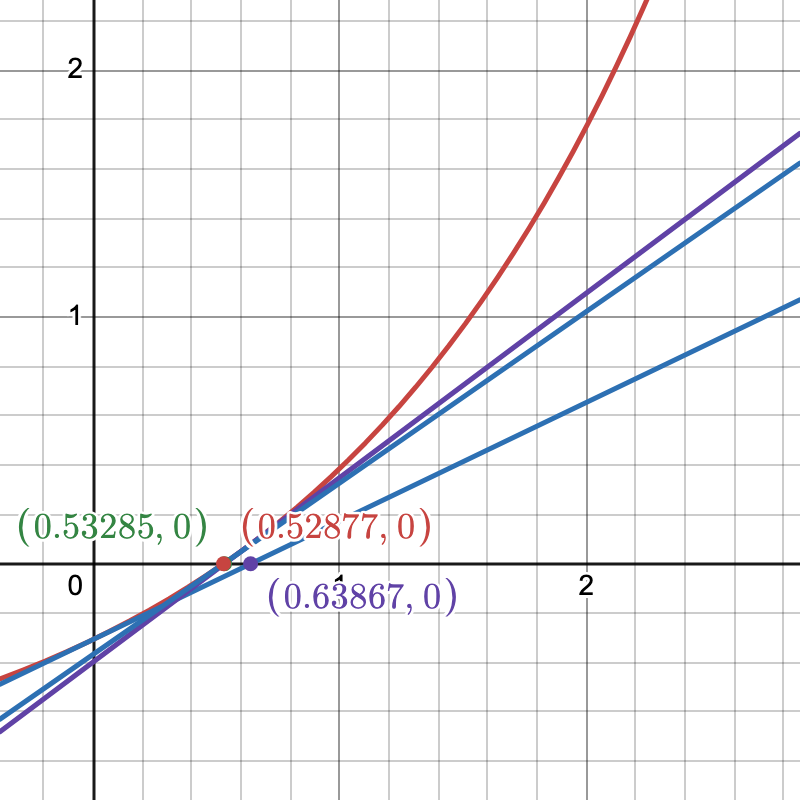
\includegraphics[width=0.7\linewidth]{HW4-1-1.png}
    \caption{Geometric interpretation of Newton's method: plot of $y=f'(x)$ and tangent lines at each iteration.}
    \label{fig:newton_geom}
\end{figure}
    
    
\end{enumerate}

\section{Nonconvex optimization}
The following problems involve optimization of nonlinear nonconvex functions with some simple constraints, such as an interval or a box in higher dimension. 
To minimize each of the following functions, you can use the command {\tt minimize} from {\tt scipy.optimize}. Due to the nonconvex and sometimes nonsmooth (i.e. not differentiable at some points) nature of the objective function, you need to be careful about the starting point and the constraints you set. For example, you may need to set the box small enough to help the solver find a good local optimum. You need to provide a printout of your code, along with the solution. 

\begin{enumerate}


\item Minimize $f(x_1, x_2)=(1-x_2+x_1x_2)^2+(2-x_2+x_1x_2^2)^2+(3-x_2+x_1x_2^3)^2$ over the box $-5\le x_1, x_2 \le 5$. Start from $(0,0)$. Plot the function $f(x_1,x_2)$ over the box $[-5,5]^2$ using both a 2D contour plot and a 3D plot.

\textbf{Solution:}

Python code and results:

\begin{verbatim}
def problem_2_1():
    """Solve problem 2.1: Minimize the given function"""
    def objective(x):
        x1, x2 = x[0], x[1]
        return (1 - x2 + x1*x2)**2 + (2 - x2 + x1*x2**2)**2 + (3 - x2 + x1*x2**3)**2
    
    # Optimization
    x0 = [0, 0]
    bounds = [(-5, 5), (-5, 5)]
    result = minimize(objective, x0, bounds=bounds, method='L-BFGS-B')
    
    print("Problem 2.1 Results:")
    print(f"Optimal solution: x1 = {result.x[0]:.6f}, x2 = {result.x[1]:.6f}")
    print(f"Optimal value: {result.fun:.6f}")
    print(f"Success: {result.success}")
    
    # Plotting
    x1 = np.linspace(-5, 5, 100)
    x2 = np.linspace(-5, 5, 100)
    X1, X2 = np.meshgrid(x1, x2)
    Z = objective([X1, X2])
    
    fig, (ax1, ax2) = plt.subplots(1, 2, figsize=(15, 6))
    
    # Contour plot
    contour = ax1.contour(X1, X2, Z, levels=20)
    ax1.clabel(contour, inline=True, fontsize=8)
    ax1.plot(result.x[0], result.x[1], 'r*', markersize=15, label='Optimal point')
    ax1.set_xlabel('x1')
    ax1.set_ylabel('x2')
    ax1.set_title('2D Contour Plot')
    ax1.legend()
    ax1.grid(True, alpha=0.3)
    
    # 3D plot
    ax2 = fig.add_subplot(122, projection='3d')
    surf = ax2.plot_surface(X1, X2, Z, cmap='viridis', alpha=0.8)
    ax2.scatter([result.x[0]], [result.x[1]], [result.fun], 
               color='red', s=100, label='Optimal point')
    ax2.set_xlabel('x1')
    ax2.set_ylabel('x2')
    ax2.set_zlabel('f(x1, x2)')
    ax2.set_title('3D Plot')
    ax2.legend()
    
    plt.tight_layout()
    plt.show()
\end{verbatim}

Results:
\begin{itemize}
\item Optimal solution: $x_1^* = -0.276725, x_2^* = 1.519078$
\item Optimal value: $f(x^*) = 1.168412$
\item Convergence: Success
\end{itemize}

For the plots, we create both 2D contour plots and 3D plots to visualize the function shape and the location of the optimal solution.

\begin{figure}[H]
    \centering
    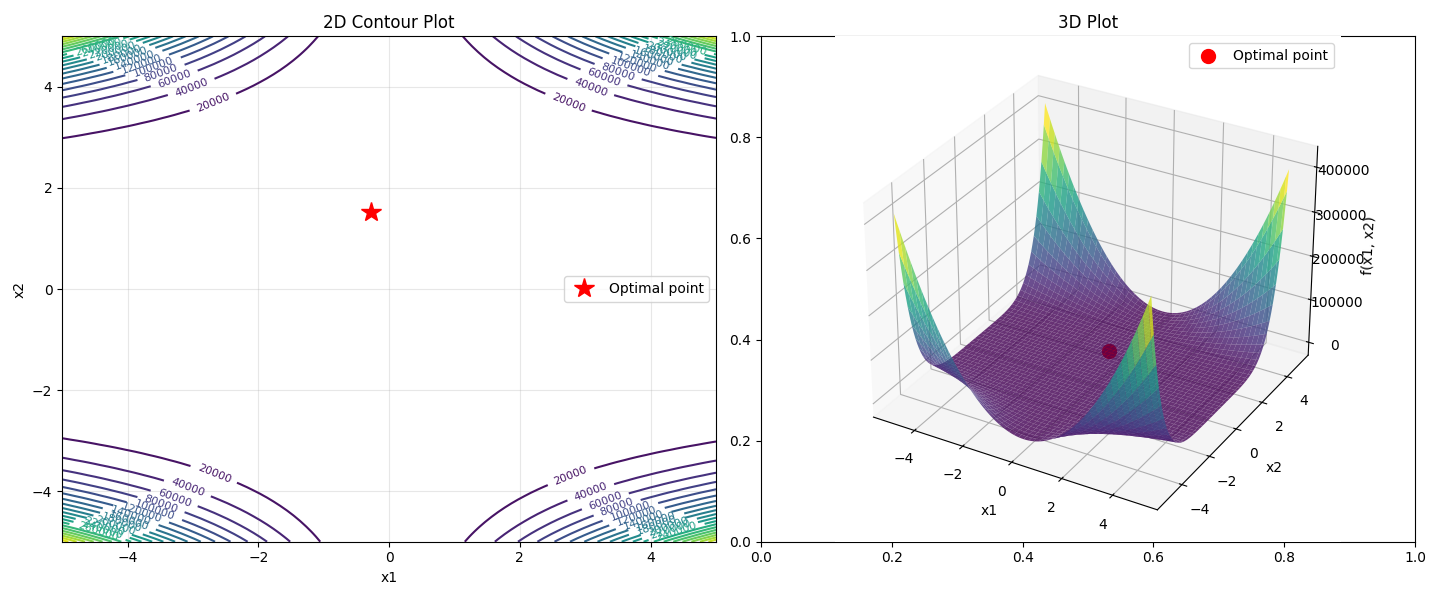
\includegraphics[width=0.8\linewidth]{Figure_2_1.png}
    \caption{2D contour plot and 3D plot of the objective function for Problem 2.1. The optimal solution is marked with a red star.}
    \label{fig:problem_2_1}
\end{figure}



\item Consider the following function:
$$f(x_1,x_2) = (2x_1 + x_2^2 - 4)^2 + (x_1^2 + x_2 - 8)^2,\ -5\le x_1,x_2 \le 5.$$ 
Try to find as many local minima as you can. Plot the function $f(x_1,x_2)$ over the box $[-5,5]^2$ using both a 2D contour plot and a 3D plot. Hint: You can start the algorithm that you choose from different starting points.

\textbf{Solution:}

Python code and results:

\begin{verbatim}
def problem_2_2():
    """Solve problem 2.2: Find multiple local minima"""
    def objective(x):
        x1, x2 = x[0], x[1]
        return (2*x1 + x2**2 - 4)**2 + (x1**2 + x2 - 8)**2
    
    # Multiple starting points
    starting_points = [
        [0, 0], [2, 2], [-2, 2], [2, -2], [-2, -2],
        [3, 3], [-3, 3], [3, -3], [-3, -3], [1, 4]
    ]
    
    bounds = [(-5, 5), (-5, 5)]
    local_minima = []
    
    print("Problem 2.2 Results:")
    for i, x0 in enumerate(starting_points):
        result = minimize(objective, x0, bounds=bounds, method='L-BFGS-B')
        local_minima.append((result.x, result.fun, result.success))
        print(f"Starting point {x0}: solution={result.x}, value={result.fun:.6f}, success={result.success}")
    
    # Remove duplicates to identify unique local minima
    unique_minima = []
    for x, val, success in local_minima:
        if success:
            is_unique = True
            for ux, uval in unique_minima:
                if np.linalg.norm(np.array(x) - np.array(ux)) < 1e-3:
                    is_unique = False
                    break
            if is_unique:
                unique_minima.append((x, val))
    
    print(f"\nNumber of local minima found: {len(unique_minima)}")
    for i, (x, val) in enumerate(unique_minima):
        print(f"Local minimum {i+1}: x1={x[0]:.6f}, x2={x[1]:.6f}, f(x)={val:.6f}")
    
    # Plotting
    x1 = np.linspace(-5, 5, 100)
    x2 = np.linspace(-5, 5, 100)
    X1, X2 = np.meshgrid(x1, x2)
    Z = objective([X1, X2])
    
    fig, (ax1, ax2) = plt.subplots(1, 2, figsize=(15, 6))
    
    # Contour plot
    contour = ax1.contour(X1, X2, Z, levels=20)
    ax1.clabel(contour, inline=True, fontsize=8)
    for i, (x, val) in enumerate(unique_minima):
        ax1.plot(x[0], x[1], 'r*', markersize=15, label=f'Local min {i+1}' if i == 0 else '')
    ax1.set_xlabel('x1')
    ax1.set_ylabel('x2')
    ax1.set_title('2D Contour Plot with Local Minima')
    ax1.legend()
    ax1.grid(True, alpha=0.3)
    
    # 3D plot
    ax2 = fig.add_subplot(122, projection='3d')
    surf = ax2.plot_surface(X1, X2, Z, cmap='viridis', alpha=0.8)
    for i, (x, val) in enumerate(unique_minima):
        ax2.scatter([x[0]], [x[1]], [val], 
                   color='red', s=100, label=f'Local min {i+1}' if i == 0 else '')
    ax2.set_xlabel('x1')
    ax2.set_ylabel('x2')
    ax2.set_zlabel('f(x1, x2)')
    ax2.set_title('3D Plot with Local Minima')
    ax2.legend()
    
    plt.tight_layout()
    plt.show()
\end{verbatim}

Results:
\begin{itemize}
\item Number of local minima found: 3
\item Local minimum 1: $x_1 = 2.698908, x_2 = 0.185260, f(x) = 2.332591$
\item Local minimum 2: $x_1 = -2.254543, x_2 = 2.917034, f(x) = 0.000000$
\item Local minimum 3: $x_1 = -3.357589, x_2 = -3.273405, f(x) = 0.000000$
\end{itemize}

For the plots, we create both 2D contour plots and 3D plots to visualize the locations of multiple local minima and the function shape.

\begin{figure}[H]
    \centering
    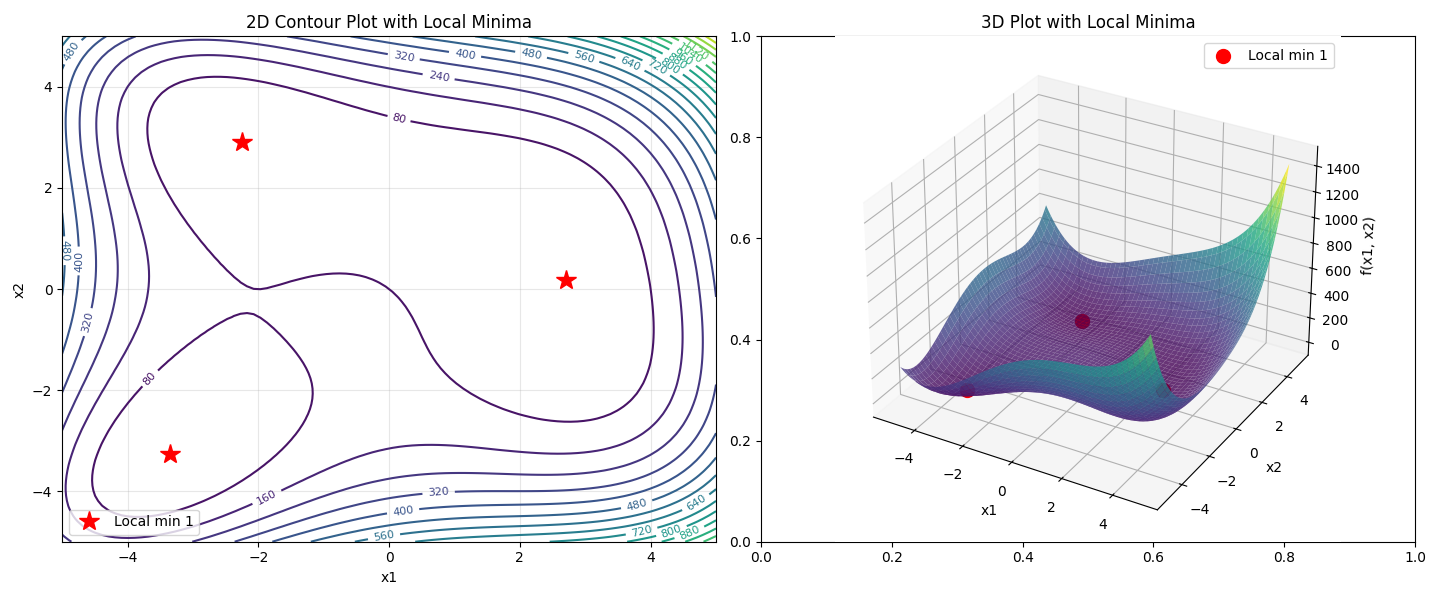
\includegraphics[width=0.8\linewidth]{Figure_2_2.png}
    \caption{2D contour plot and 3D plot of the objective function for Problem 2.2. Multiple local minima are marked with red stars.}
    \label{fig:problem_2_2}
\end{figure}


\end{enumerate}
\end{document}